
% this file is called up by thesis.tex
% content in this file will be fed into the main document

%: ----------------------- introduction file header -----------------------
\begin{savequote}[50mm]
The logic of validation allows us to move between the two limits of dogmatism and skepticism. 
\qauthor{Paul Ricoeur}
\end{savequote}


\chapter{Evaluación}
\label{cha:Validation of the methodology}

% the code below specifies where the figures are stored
\ifpdf
    \graphicspath{{5_experiments_and_results/figures/PNG/}{5_experiments_and_results/figures/PDF/}{5_experiments_and_results/figures/}}
\else
    \graphicspath{{5_experiments_and_results/figures/EPS/}{5_experiments_and_results/figures/}}
\fi


%------------------------------------------------------------------------- 

En este capítulo se evalúa la idoneidad del método propuesto para la evaluación de competencias genéricas. Este capítulo se estructura de la siguiente manera:

\section{Introducción}

	bla bla bla

\section{Herramientas}

	bla bla bla

	\subsection{Antecedentes}

	El uso educacional de los wikis para las experiencias de trabajo colaborativo está en auge debido a las numerosas ventajas que aporta sobre los modelos tradicionales~\cite{elgort2008wiki}. Algunas de las ventajas sobre los medios tradicionales, ya sean en formato impreso o en documentos digitales, es que éstos no llevan un registro de ediciones, no permiten la colaboración distribuida y asíncrona y no pueden ser monitorizados por el profesor mientras los estudiantes completan el trabajo.

	Para evaluar el trabajo final de un grupo de estudiantes en una página del wiki nos bastaría con leer la última versión de dicha página, como hacíamos con los métodos tradicionales. Pero una de las características más interesantes de los wikis es que no sólo almacenan la información de la versión final de cada documento, sino que también almacenan todas las versiones intermedias creadas como resultado de las contribuciones hechas por cada usuario~\cite{trentin2009using}. Esto lo consigue manteniendo un registro con las diferencias entre las ediciones consecutivas de las páginas, registro que se podría utilizar para la obtención de indicadores de diferentes competencias~\cite{ortega2011new}. Las páginas creadas de manera colaborativa podrían ser evaluadas considerando la contribución de cada autor y las dinámicas de grupo en la creación de la página en tiempo real. Por desgracia, realizar una evaluación detallada de cada contribución realizada en el wiki es imposible de abordar cuando hay muchos usuarios y éstos participan activamente.

	En un proyecto anterior, para poder evaluar el trabajo de los estudiantes en las páginas de un wiki se desarrolló \emph{StatMediaWiki} (SMW)~\footnote{http://statmediawiki.forja.rediris.es/}, una herramienta que proporciona al profesor información cuantitativa sobre la distribución del trabajo de los estudiantes en las páginas del wiki, es decir, qué parte del trabajo realizado en una página del wiki corresponde a cada estudiante~\cite{duarte2012wikis}.  A partir de esa información cuantitativa se midieron las competencias de la adaptación al cambio, el trabajo en equipo, el aprendizaje y la innovación. Sin embargo, el aspecto cualitativo quedó fuera, ya que el experimento sólo consideró el número, el momento y el tamaño de las contribuciones~\cite{palomo2014assessment}.

	Para completar el análisis cuantitativo proporcionado por SMW con un análisis cualitativo y medir el desempeño en otras competencias genéricas se desarrolla \emph{AssessMediaWiki} (AMW)~\footnote{http://assessmediawiki.forja.rediris.es}. AMW es una herramienta para realizar una evaluación escalable y cualitativa del trabajo realizado en el wiki mediante procedimientos de autoevaluación, evaluación entre iguales y evaluación del profesor.

		\subsubsection{AssessMediaWiki (AMW)}

		AMW es una aplicación web de código abierto que, al conectarse a una instalación MediaWiki, proporciona procedimientos de autoevaluación, evaluación entre iguales y evaluación del profesor, a la vez que mantiene información sobre esas evaluaciones. AMW pone a disposición de los estudiantes una rúbrica previamente definida por el profesor para que realicen la evaluación (figura\ref{fig:AmwRubrica}). 

\begin{figure}
  \begin{center}
    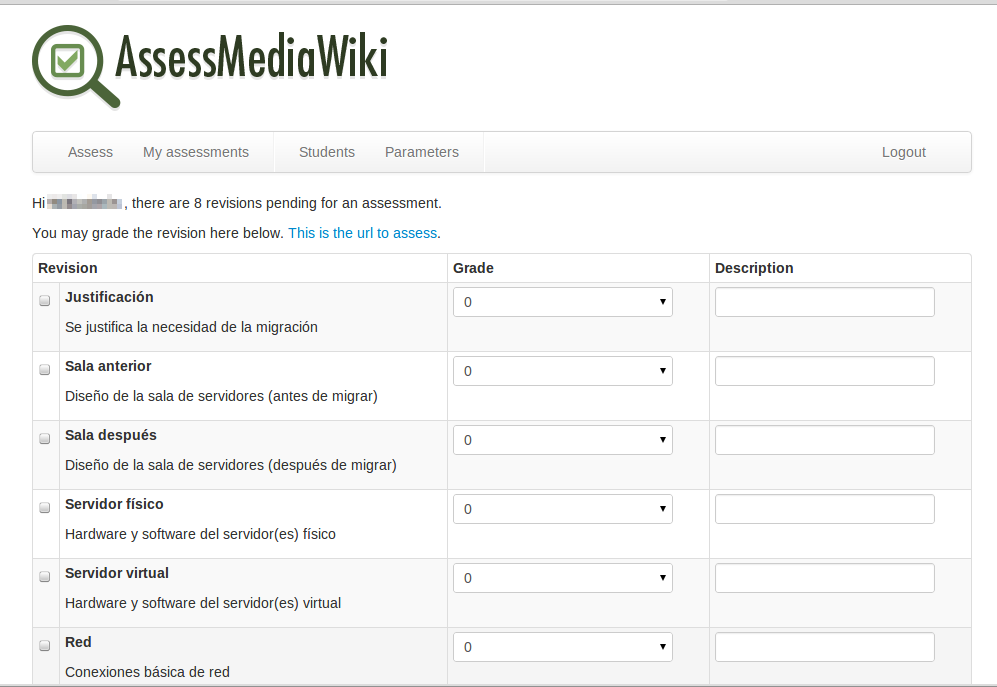
\includegraphics[scale=0.3]{AmwRubrica.png}
  \end{center}
  \caption{Rúbrica de AMW}
  \label{fig:AmwRubrica}
\end{figure}

		AMW implementa dos roles de usuario distintos: supervisores y estudiantes. Los estudiantes pueden elegir entre distintas opciones: evaluar una revisión, comprobar sus propias aportaciones evaluadas y verificar las evaluaciones ya enviadas. Por otro lado, los supervisores tienen un mayor número de opciones, como definir la rúbrica que los estudiantes deberán completar al realizar sus evaluaciones, modificar los parámetros de los programas o vigilar las evaluaciones que los alumnos vayan haciendo. AMW implementa una función de selección parcialmente aleatoria. Cuando un estudiante va a realizar una evaluación, el sistema elige automáticamente una de entre el 30\percentage más significativa que aún no ha sido evaluada.

		Al revisar sus evaluaciones, los estudiantes puede revisar las notas recibidas y sus justificaciones, así como ver a qué contribución en particular se refiere (figura~\ref{fig:AmwFormative}). Si el estudiante no está de acuerdo con la calificación puede replicar utilizando para ello una rúbrica similar a la que se utilizó en su evaluación, indicando las calificaciones que considera que merece y sus correspondientes justificaciones. Después el profesor revisará la disputa y pondrá la nota definitiva.

\begin{figure}
  \begin{center}
    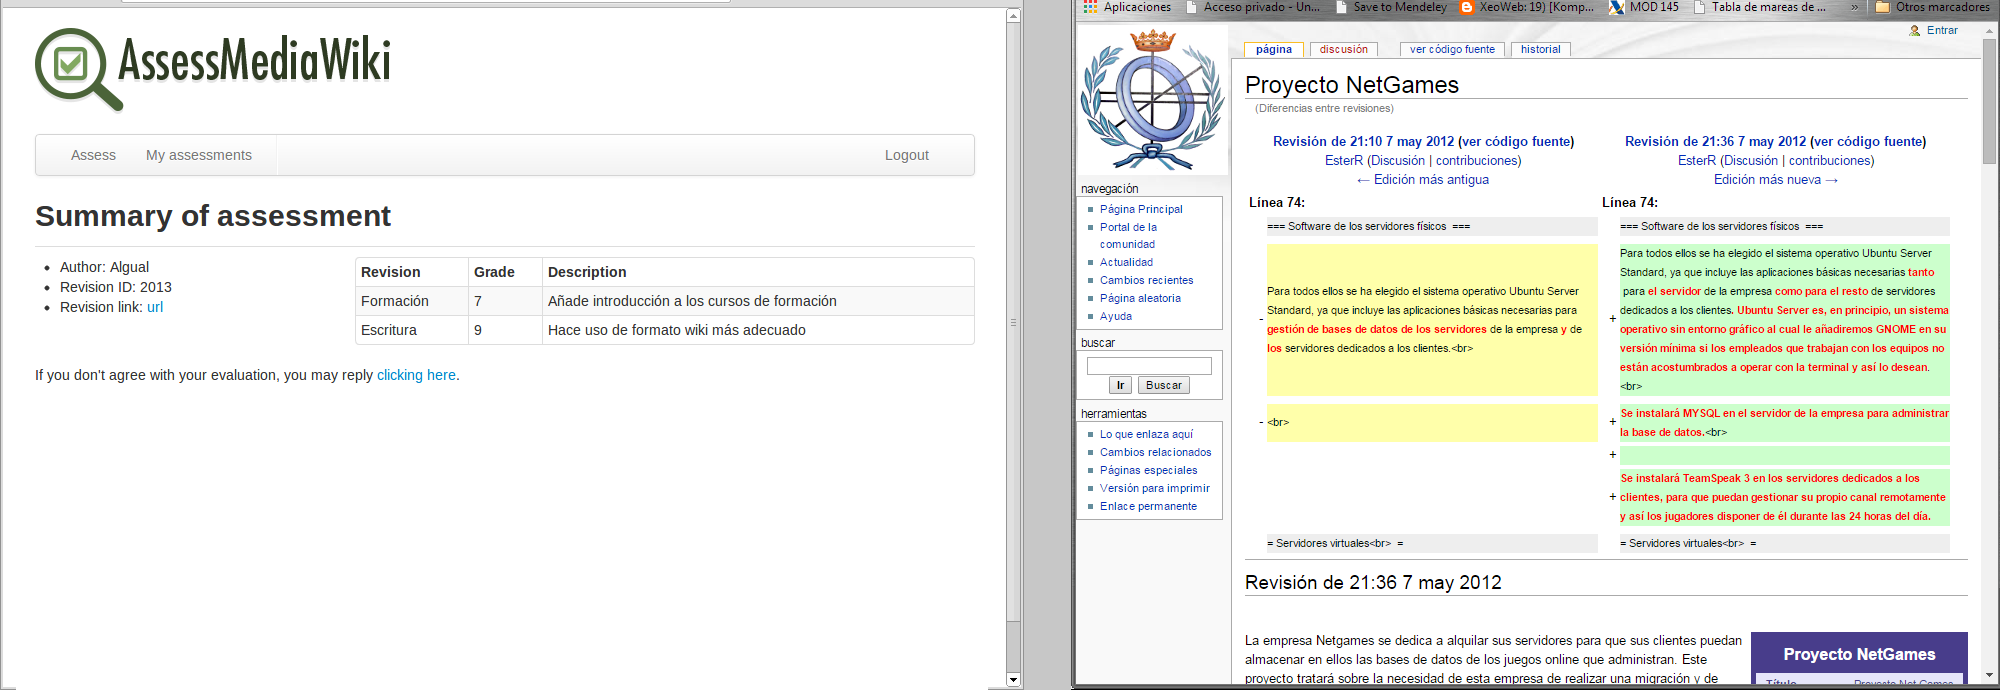
\includegraphics[scale=0.19]{AmwFormative.png}
  \end{center}
  \caption{Ejemplo de retroalimentación formativa y la contribución de wiki evaluada}
  \label{fig:AmwFormative}
\end{figure}

			\paragraph{Ejemplo de uso}

			El método para la evaluación del trabajo y las competencias desempeñadas en el wiki consta de dos partes: una primera parte en la que lo que se evalúa es el trabajo del wiki (A), basada en procedimientos de autoevaluación, evaluación entre iguales y evaluación del profesor; y una segunda parte en la que se evalúan las competencias genéricas (B) y en la que se pone en práctica el \emph{ciclo de contraste de hipótesis}.

			\paragraph*{A. Evaluación del trabajo en el wiki.}

			El método para la evaluación del trabajo en el wiki se divide también en tres fases: una primera fase en la que los estudiantes realizan sus trabajos en las páginas del wiki, una segunda fase de evaluación y una tercera fase de revisión del profesor. En la figura~\ref{fig:AmwDiagram} puede verse un diagrama de flujo de trabajo que muestra cada una de las fases del método de evaluación realizado sobre una página del wiki en la que participan varios estudiantes y el profesor. A continuación se describen cada una de estas fases.

\begin{figure}
  \begin{center}
    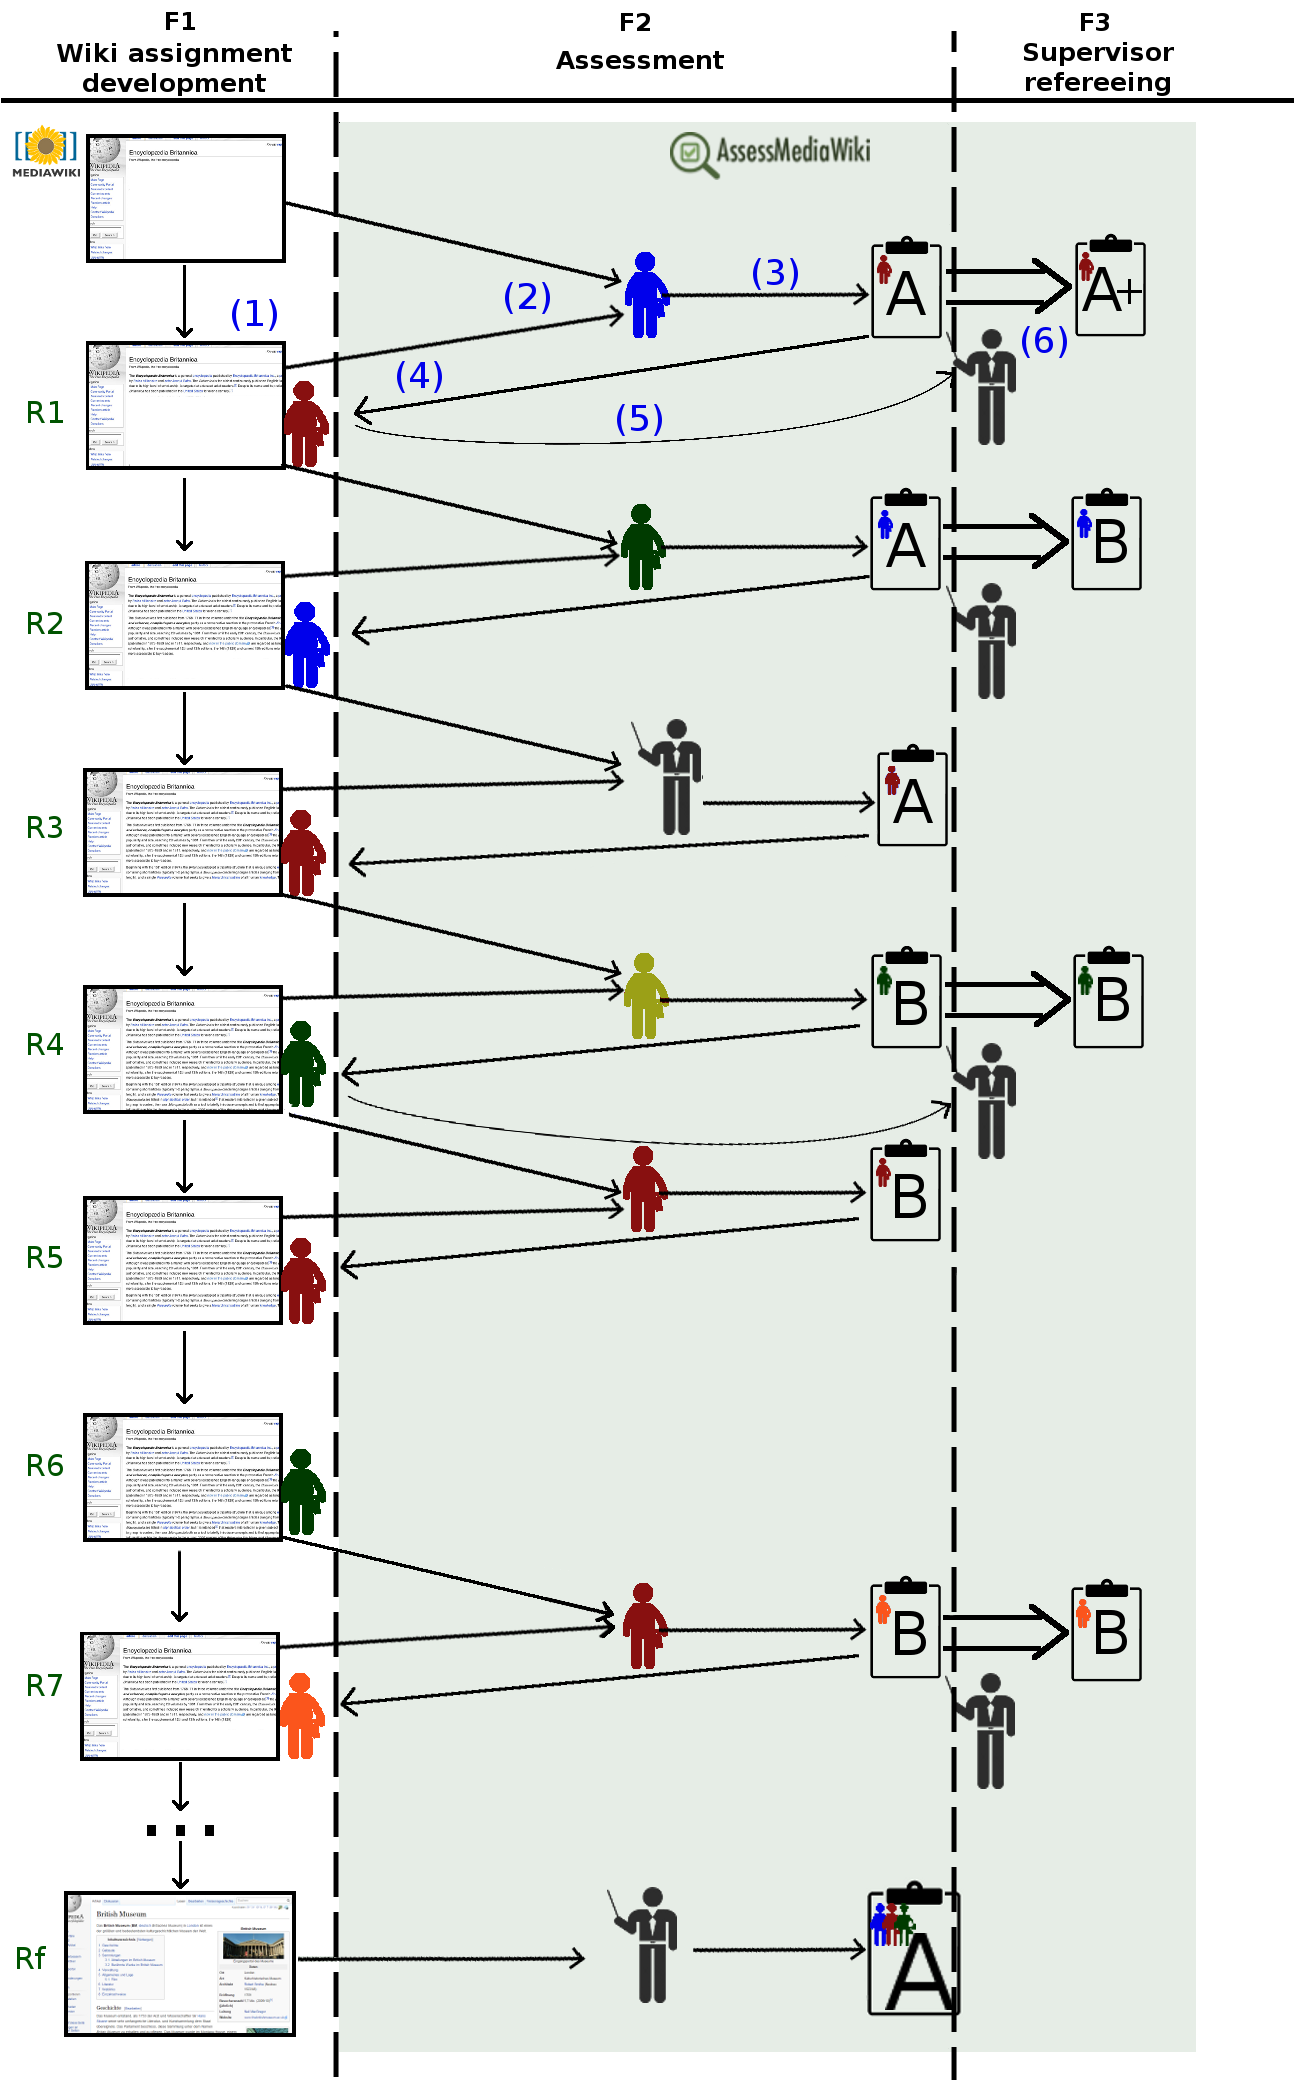
\includegraphics[scale=0.28]{AmwDiagram.png}
  \end{center}
  \caption{Ejemplo de flujo de trabajo para la evaluación cualitativa del wiki utilizando AMW}
  \label{fig:AmwDiagram}
\end{figure}

			\subparagraph*{Fase 1: Desarrollo del trabajo en el wiki.}

			Esta fase se representa en la columna de la izquierda de la figura~\ref{fig:AmwDiagram}, y es en la que los estudiantes realizan el trabajo en las páginas del wiki. Normalmente, cada grupo de estudiantes tendrá que desarrollar su trabajo en una página del wiki. En la zona más alta de la columna se representa el comienzo del trabajo con una página en blanco. El autor de cada contribución se muestra con una figura de color junto a la misma. Para comenzar, el usuario de color rojo crea una página vacía (\emph{R1}). Después, el usuario azul añade contenido a la página (\emph{R2}). En tercer lugar, el usuario rojo modifica de nuevo la página añadiendo texto a la versión dejada anteriormente por el usuario azul (\emph{R3}) y así sucesivamente. Esta fase termina cuando llega la fecha marcada por el profesor para que los trabajos estén finalizados (\emph{Rf} es la versión final de la página).

			Puede verse que, aunque los estudiantes responsables de la página de ejemplo del wiki fuesen el rojo, el azul y el verde, otros estudiantes, como el naranja en la revisión séptima, podrían contribuir a la página del wiki. En ese caso, los miembros del grupo y responsables de la página deben decidir si la contribución debe conservarse o no.

			\subparagraph*{Fase 2: Evaluación.}

			Esta fase se muestra en la columna central y comprende las siguientes actividades:

			\begin{itemize}
				\item \emph{Autoevaluación, evaluación entre iguales y evaluación del profesor}. Las contribuciones a ser evaluadas se asignan a los estudiantes.  Cada contribución es la diferencia entre dos revisiones consecutivas de una página del wiki. El estudiante encargado de evaluar dicha contribución se representa en el gráfico como un usuario coloreado que recibe dos flechas de las revisiones, una de la revisión anterior a la contribución y otra de la revisión que incorpora ya la contribución. Para la evaluación los estudiantes utilizan una rúbrica definida por el profesor. Cada contribución sólo se refiere a una contribución atómica de las realizadas a una página del wiki por un único estudiante, por lo que dicha contribución podría ser utilizada como un indicador de la contribución al wiki de dicho estudiante. El estudiante que realizó cada contribución se representa con una figura pegada a la revisión de la página en cada momento.
Por ejemplo, en la primera evaluación, se asigna la contribución realizada a la página del wiki por el estudiante rojo (\emph{1}) al estudiante azul. El estudiante azul comprueba ambas versiones para ver las diferencias entre ambas versiones (\emph{2}) y realiza la evaluación completando la rúbrica proporcionada por el profesor (\emph{3}).
Cabe destacar también otras situaciones interesante. En la versión \emph{R5} de la página vemos como se realiza una autoevaluación, ya que el estudiante rojo, autor de la versión, es el mismo que tiene que evaluar su contribución. Vemos también que en \emph{R3} es el profesor el que realiza la evaluación de la contribución del estudiante rojo. Esto puede deberse a que el estudiante manualmente detecta una contribución que considera oportuna evaluar o a que, utilizando la herramienta SMW, detecta un comportamiento extraño en el wiki y quiere contrastar la situación. 
Puede verse también que hay contribuciones que no reciben evaluación alguna, como ocurre con \emph{R6}. Está claro que sería deseable que todas las contribuciones significativas fueran evaluadas, pero no es escalable.
				\item \emph{Revisión de las evaluaciones recibidas}. Los estudiantes pueden revisar las evaluaciones recibidas. Ellos pueden no sólo ver las notas que han recibido con las justificaciones y comentarios que añadieron sus evaluadores, sino también el enlace a la contribución. De esta forma, los estudiantes evaluados reciben una retroalimentación formativa. En la primera de las evaluaciones del diagrama de ejemplo puede verse como el estudiante rojo puede ver su evaluación (\emph{4}).
				\item \emph{Réplica}. Si el estudiante evaluado no está de acuerdo con la evaluación recibida tiene la opción de replicarla justificando el motivo de dicha réplica. En el diagrama de ejemplo puede verse como el estudiante rojo considera injusta su evaluación y realiza una réplica (\emph{5}). El profesor deberá resolver la réplica en la siguiente etapa.
				\item \emph{Evaluación final del wiki}. El profesor evalúa la versión final de la página del wiki desarrollada por cada grupo de estudiantes. Esta evaluación es necesaria ya que el objetivo principal de la tarea es que los estudiantes realicen un buen trabajo en una página del wiki. Como cualquier otra tarea, deberá ser evaluada por el profesor conforme al programa de estudios. Además, algunos de los criterios de evaluación sólo pueden ser evaluados en la versión final de la página, como por ejemplo, la coherencia del texto. De esta forma, aquellas contribuciones del wiki descartadas por la función de selección serán ahora implícitamente evaluadas ya que están integradas en el entregable final. Puede verse la evaluación al final del diagrama de ejemplo (\emph{Rf}), y cómo afecta al grupo de estudiantes completo.
\end{itemize}

			El diagrama no recoge algunas situaciones que también podrían darse. Por ejemplo, alguna contribución podría ser evaluada por más de un usuario, ya fuera otro estudiante o el profesor. También, para simplificar, el diagrama sólo muestra una calificación para la contribución (A, A+, B, ... etc.), pero las evaluaciones son multidimensionales.

			Un componente interesante de nuestro algoritmo es qué contribución wiki podrá ser asignada a cada estudiante para su evaluación. Es lo que llamamos \emph{función de selección}, y tiene varios aspectos a tener en cuenta:

			\begin{itemize}
				\item \emph{¿Debería cierta contribución en el wiki ser evaluada por más de un estudiante?} En realidad, tener varias evaluaciones de estudiantes diferentes sobre una misma contribución podría ser interesante para perfeccionar su evaluación y podría proporcionar información al profesor para evaluar no sólo al estudiante autor de la contribución, sino también a los evaluadores. De hecho, el número de contribuciones a ser evaluadas es dependiente del objetivo del experimento y su configuración. Cuánto más grande sea el experimento, más contribuciones susceptibles de ser evaluadas tendrá. Sin embargo, el número de evaluaciones que un estudiante puede realizar es limitado (para que siga siendo formativo). Por lo que cada evaluación adicional a la misma contribución provocará que otras contribuciones sean más pobremente evaluadas o que no lo sean.
				\item \emph{¿Qué contribuciones deberían ser evaluadas?} La importancia de evaluar cada contribución puede variar. Por ejemplo, evaluar al menos una mínima cantidad de contribuciones por cada estudiante, página o categoría sería interesante. Pero algunas contribuciones que añadan ciertas características al trabajo pueden ser relevantes o informativas sobre el trabajo realizado por un estudiante. Por ejemplo, aunque las contribuciones que añadan gran cantidad de texto suelan ser más interesantes que las contribuciones pequeñas, una contribución pequeña puede ir relacionada con el cambio de sentido de alguna frase o párrafo. De cualquier forma, un estudiante puede solicitar que una contribución en particular sea evaluada, aunque ésta quede fuera de la función de selección.
				\item \emph{¿Quién evalúa cada contribución?} Depende de la importancia que se quiera dar a la autoevaluación, la evaluación del compañero y la del profesor. De nuevo, se debería balancear el esfuerzo requerido y el detalle a exigir en las evaluaciones.
			\end{itemize}


			\subparagraph*{Fase 3: Revisión del profesor.}

			En esta última columna se representan dos actividades que corresponden al profesor:

			\begin{itemize}
				\item Resolución de las réplicas: el profesor revisa las réplicas indicando si proceden o no. En caso de que procedan, modifica la calificación. En el diagrama se puede ver como en la primera contribución, el estudiante rojo realiza una réplica (\emph{5}) sobre la evaluación reciba por el usuario azul (\emph{3}). El profesor revisa la réplica, la considera apropiada y modifica la calificación (\emph{6}). En un segundo ejemplo, en la evaluación realizada por el estudiante de color amarillo sobre la contribución realizada por el usuario de color verde puede verse como el profesor no acepta la réplica realizada por este último, y mantiene la calificación otorgada inicialmente por el estudiante amarillo.
				\item Revisión de evaluaciones no replicadas: el profesor puede revisar aleatoriamente otras evaluaciones realizadas por los estudiantes que no hayan sido replicadas. En el diagrama puede verse como en el profesor revisa las evaluaciones realizadas sobre las contribuciones representadas en \emph{R2} y en \emph{R7}, disminuyendo la calificación de la primera y manteniendo la segunda.
			\end{itemize}

			\paragraph*{B. Evaluación de competencias genéricas}

			El método para la evaluación de competencias genéricas se basa en el \emph{ciclo de contraste de hipótesis}. En la figura~\ref{fig:AmwDiagram2} puede verse la descripción del ciclo. Esta evaluación se puede llevar a cabo durante o después de que los estudiantes hayan realizado su trabajo en el wiki y sus evaluaciones con AMW. Evidentemente, cuánto más avanzado esté el trabajo más datos habrá para analizar. 

			El ciclo comienza con el diseño de un indicador por parte del profesor que podría plasmar en una hoja de cálculo a partir de los datos que recibirá de las evaluaciones (a). A continuación, el profesor realiza la petición a AMW que le proporcionará los datos (b). AMW consulta y procesa los datos en las bases de datos de MediaWiki y AMW (c) y se los envía al profesor (d). El profesor los integra en la hoja de cálculo previamente diseñada y los analiza (e). Si son válidos para la evaluación finaliza el proceso (f). Por el contrario, si necesitan algún tipo de refinamiento el profesor puede rediseñar la evaluación (g) y hacer una nueva petición.

\begin{figure}
  \begin{center}
    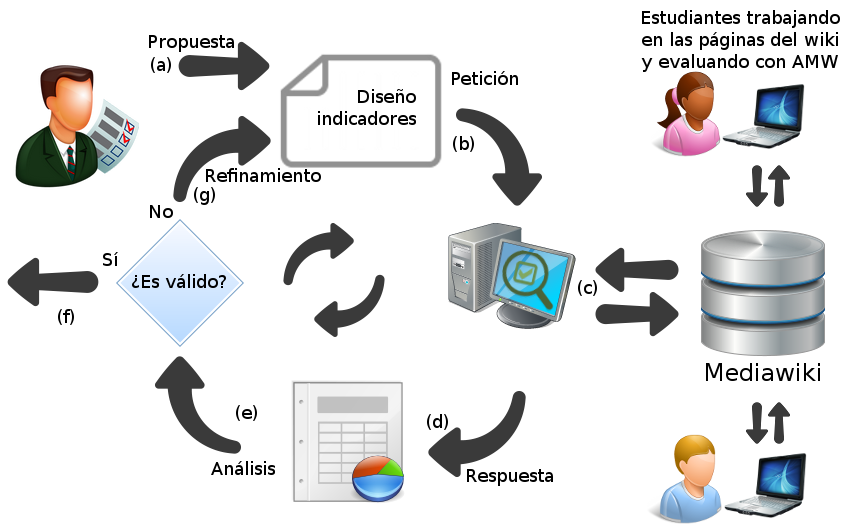
\includegraphics[scale=0.45]{AmwDiagram2.png}
  \end{center}
  \caption{Ciclo de contraste de hipótesis para la evaluación en wikis}
  \label{fig:AmwDiagram2}
\end{figure}

			\paragraph*{Indicadores de competencias genéricas}

				Los indicadores que se mencionan en este punto han sido utilizados en los estudios de caso realizados para este trabajo, pero como se ha mencionado desde un primer momento, este método proporciona indicadores y es el profesor el que los utilizará para evaluar las competencias genéricas que considere oportunas.

			\subparagraph*{Trabajo en equipo.}
			El indicador considerado para el trabajo en equipo es el \emph{ratio de miembros del equipo que trabajaron en un mismo criterio.} La rúbrica que utilizan los estudiantes para evaluar se compone de un conjunto de criterios. Cada criterio puede hacer referencia a una parte del trabajo. En todas las ediciones de un wiki no se trabajan en las mismas partes del trabajo, por lo que al ser evaluado, un estudiante puede tener nota en unos criterios y no tenerla en otros. Si más de un estudiante ha trabajado en la misma parte de una página wiki y su aportación ha sido significativa, tendrán nota en dicho criterio. Por tanto, partiendo de la cantidad de criterios que tiene un trabajo y del ratio de miembros del equipo que ha trabajado en cada criterio tendremos un indicador del trabajo en equipo.

			\subparagraph*{Comunicación y aplicación del conocimiento.}
			El indicador considerado para la comunicación y la aplicación del conocimiento es la \emph{media de las notas recibidas por todos los miembros del grupo}. Este indicador mide la incidencia que tuvieron las contribuciones realizadas en el éxito del proyecto. Una calificación pobre en una contribución puede significar  que alguna contribución wiki obtuvo una buena nota en un cierto criterio de la rúbrica pero una mala nota en el otro (el autor de la contribución soluciona un problema y crea uno nuevo). Probablemente, esto se debió a una mala comunicación entre los miembros del equipo o poco compromiso de un determinado alumno en el objetivo global del grupo. 

			\subparagraph*{Mantener la calidad del trabajo producido.}
			El indicador considerado para el mantenimiento de la calidad del trabajo producido es la \emph{media de las notas que cada estudiante individualmente recibió}. Unas calificaciones altas en las evaluaciones recibidas pueden significar que el trabajo que el estudiante está produciendo es de calidad. Si el estudiante produjese mucho contenido, pero este no fuese de calidad, las calificaciones no serían buenas. Es decir, sus calificaciones están teniendo en cuenta el aspecto cualitativo del trabajo y por tanto una nota alta significaría un trabajo de calidad.

			\subparagraph*{Capacidad crítica.}
			El indicador considerado para la capacidad crítica es el \emph{número de evaluaciones que el estudiante realizó con respecto al número de dichas evaluaciones cuya nota fue modificada por el profesor}. Este indicador mide la competencia de un estudiante para evaluar el trabajo hecho por otros. Si recibiera un número fijado de réplicas en sus revisiones y estas fueran revisadas por el profesor modificando las calificaciones, podríamos considerar que dicho alumno no ha desempeñado bien dicha competencia.

			En la tabla~\ref{tab:ResumenIndicadoresCualiCuanti} puede verse una comparación entre los indicadores considerados a partir de la evaluación cualitativa que se realizaría con AMW y los que se obtienen a partir de la evaluación cuantitativa realizada con SMW.

\begin{table}
  \begin{center}
  \begin{tabular}{| m{3.2cm} | m{4.9cm} | m{5.1cm} |}
    \hline 
    \multirow{2}{*}{COMPETENCIAS}  & INDICADORES  & INDICADORES  \\
      &  CUALITATIVOS  &  CUANTITATIVOS \\
    \hline
    \hline
    Trabajo en equipo  & Ratio de miembros del equipo que trabajaron en un mismo criterio  & Ratio de miembros del equipo que contribuyeron a una misma página del wiki en las páginas de su proyecto \\
    \hline
    Comunicación y aplicación del conocimiento  & Media de las notas recibidas por todos los miembros del grupo  & Porcentaje de miembros del equipo que contribuyeron al menos a un 20\percentage del trabajo realizado \\
    \hline
    Mantener la calidad del trabajo producido  & Media de las notas que cada estudiante individualmente recibió  & Contribución individual en bytes \\
    \hline
    Capacidad crítica  & Número de evaluaciones que el estudiante realizó con respecto al número de dichas evaluaciones cuya nota fue modificada por el profesor  & No considerada \\
    \hline
  \end{tabular}
\end{center}
\caption{Resumen de las competencias evaluadas para cada tipo de indicador}
\label{tab:ResumenIndicadoresCualiCuanti}
\end{table}

			\paragraph{Conclusiones}

			AMW es una herramienta de evaluación asistida que proporciona un análisis cualitativo interesante, pues al análisis cuantitativo proporcionado por StatMediWiki, se podría añadir una información cualitativa que impidiera el engaño de los estudiantes. Por ejemplo, la contribución de un estudiante que copiase y pegase una gran cantidad de texto en una página del wiki sería considerada a efectos cuantitavos como una contribución de peso. Sin embargo, desde un punto de vista cualitativo, podría detectarse que la contibución había sido plagiada de internet con el fin de engañar al sistema.

			Sin embargo, en la aplicación de AMW nos encontramos con que se dan algunos de los problemas detectados en la revisión de la literatura para este tipo de herramientasde evaluación asistida. En primer lugar, delegar la evaluación en los estudiantes genera situaciones de subjetividad, pues pueden existir apartados en la rúbrica que los estudiantes interpreten o valoren de forma diferente. Y en segundo lugar, como vemos en el diagrama, el profesorado también revisa las evaluaciones de sus estudiantes, y más aun si estos replican, con lo que los problemas de escalabilidad también aparecerían.

	\subsection{DSL}

		Un DSL es un pequeño lenguaje de programación de gran potencia expresiva que se enfoca a un dominio particular. Los beneficios de utilizar un DSL son~\cite{vanDeursen:2000}:
		\begin{itemize}
			\item La solución a los problemas pueden ser expresados en un idioma y al nivel de abstracción del dominio del problema, y como consecuencia, los expertos en el dominio pueden entenderlo, validarlo, modificarlo y desarrollar sus propias soluciones.
			\item Los programas son concisos, autodocumentados en gran medida y reutilizables para diferentes propósitos.
			\item Mejora la productividad, la fiabilidad, la mantenibilidad y la portabilidad.
			\item Permite la validación y optimización al nivel del dominio.
			\item Mejora la capacidad de ser probado.
		\end{itemize} 

		La primera propuesta de DSL se aplica a los cursos virtuales. El VLE es el núcleo de los cursos virtuales, donde los profesores ponen el material a disposición de los estudiantes y donde los estudiantes pueden fácilmente acceder a ellos; donde tanto los profesores como los estudiantes se pueden comunicar entre ellos de manera síncrona y asíncrona; y donde los estudiantes gestionan sus proyectos en equipo mientras dialogan entre ellos. Gracias a la gran cantidad de información que genera la actividad de los estudiantes y que queda registrada en el VLE, los investigadores de diferentes áreas han colaborado para extraerlos, realizar minería de datos y utilizarlos para mejorar el aprendizaje~\cite{park2015development}.

		Además, en algunos de los trabajo recopilados en el estado del arte mostrado en el capítulo~\ref{cha:State of the Art}, se confirma la relación entre la interacción que llevan a cabo los estudiantes en el VLE y su rendimiento en el desempeño de varias competencias genéricas~\cite{fidalgo:2015,rayon2014web}. 

		\subsubsection{EvalCourse (EVC) y SASQL}

		\subsubsection{EvalSim}

			bla bla bla

\section{Estudios de caso}

	bla bla bla

	\subsection{Procesadores de Lenguajes II}

		bla bla bla

	\subsection{Programación Funcional}

		bla bla bla

	\subsection{Alemán como lengua extranjera}

		bla bla bla

	\subsection{Actuación avalada}

		bla bla bla

\section{Validación (INVESTIGAR TÍTULO ADECUADO)}

	bla bla bla

	\subsection{Curso wiki innovación}

		8 cuestionarios

	\subsection{Taller Aulablog}

		14 cuestionarios

	\subsection{Actuación avalada}

		8 cuestionarios

	\subsection{Mediawiki España}

		19 cuestionarios

\section{Difusión}

	bla bla bla

	\subsection{AssessMediaWiki}

		Conferencia: SPDECE 2012; y revista: CHB, 2012

	\subsection{EvalCourse}

		Conferencias: EC-TEL 2013, ISELEAR 2013 y SIIE 2014; Revista: IJEE, 2015

	\subsection{EvalSim}

		Conferencias: ISELEAR 2015; Revista: JITR, 2016

\section{Conclusiones}

	bla bla bla